\section{Robotics and AI in Ocean Observation}

The use of mobile robotic assets in ocean observation is relatively
recent. While research related to atmospheric phenomenon has long
leveraged technology including remote sensing satellites, generating
ocean measurements has been substantially more
challenging. Observations from satellites cannot penetrate more than a
few centimeters from the surface, sunlight does not permeate beyond
the photic zone and crushing pressure requires instrumentation to be
simple to operate yet robust to be able to survive. Terrestrial
techniques in robot sensing and perception typically do not translate
into making oceanographic measurements. 

The advent of lagrangian floats initiated the development of
untethered devices, initially to measure sub-surface currents in the
ocean via ocean acoustics. By being neutrally buoyant, these
Lagrangian devices could then float with the current and periodically
reach the surface, by changing their buoyancy, to communicate data and
then return subsurface. Variations of float designs evolved into the
design of an underwater glider with wings, a buoyancy engine and a
method to shift weights to deal with pitch and yaw motion; this work
was led by Doug Webb and Russ Davis \cite{davis02} motivated by a
seminal article by Hank Stommel who imagined how glider fleets could
traverse the worlds oceans over months making measurements while
surveying vast stretches of the ocean \cite{stomme89}. While propelled
vehicles were experimented upon as engineering artifacts
\cite{blidberg01}, glider development for scientific exploration
provided a filip to the use of AUVs.

While we are still at early stages of development of such platforms,
with sufficient computational and energy resources, yet their adoption
for science has proven to be surprisingly quick. Early adoption of
such 'robotic' vehicles from floats and gliders were traditionally
driven by the study of ocean physics (the study of currents,
acoustics, wind and the impact of bathymetry and surface
topology). More recent efforts however, have seeped into ocean biology
with the use of physical measurements as a means to understand the
presence and community structure of organisms from the micro to the
macro and highly inter-disciplinary studies of ecology of the coastal
as well as the deep ocean, thereby merging observations in physical
and bio-geochemical oceanography as a means to study ecosystems,
typically at the meso-scale. The emergence of ocean remote sensing has
also provided an inordinate amount of information about the upper
ocean, in ways that have previously been challenging to obtain,
especially at large spatio-temporal scales. Together, this has
resulted in the possibility of defining a new paradigm of ocean
observation and consequently of marine robotics. While the latter has
also had a profound impact from commercial Oil and Gas exploration
(especially with the advancement of tethered remotely operated
vehicles) and maritime defence, as also the use of \emph{immobile}
Eulerian 'robots' such as moored surface and sub-surface buoys, our
focus in this work is geared towards civilian oceanographic
observations using mobile platforms.


\begin{figure}[!t]
  \centering
  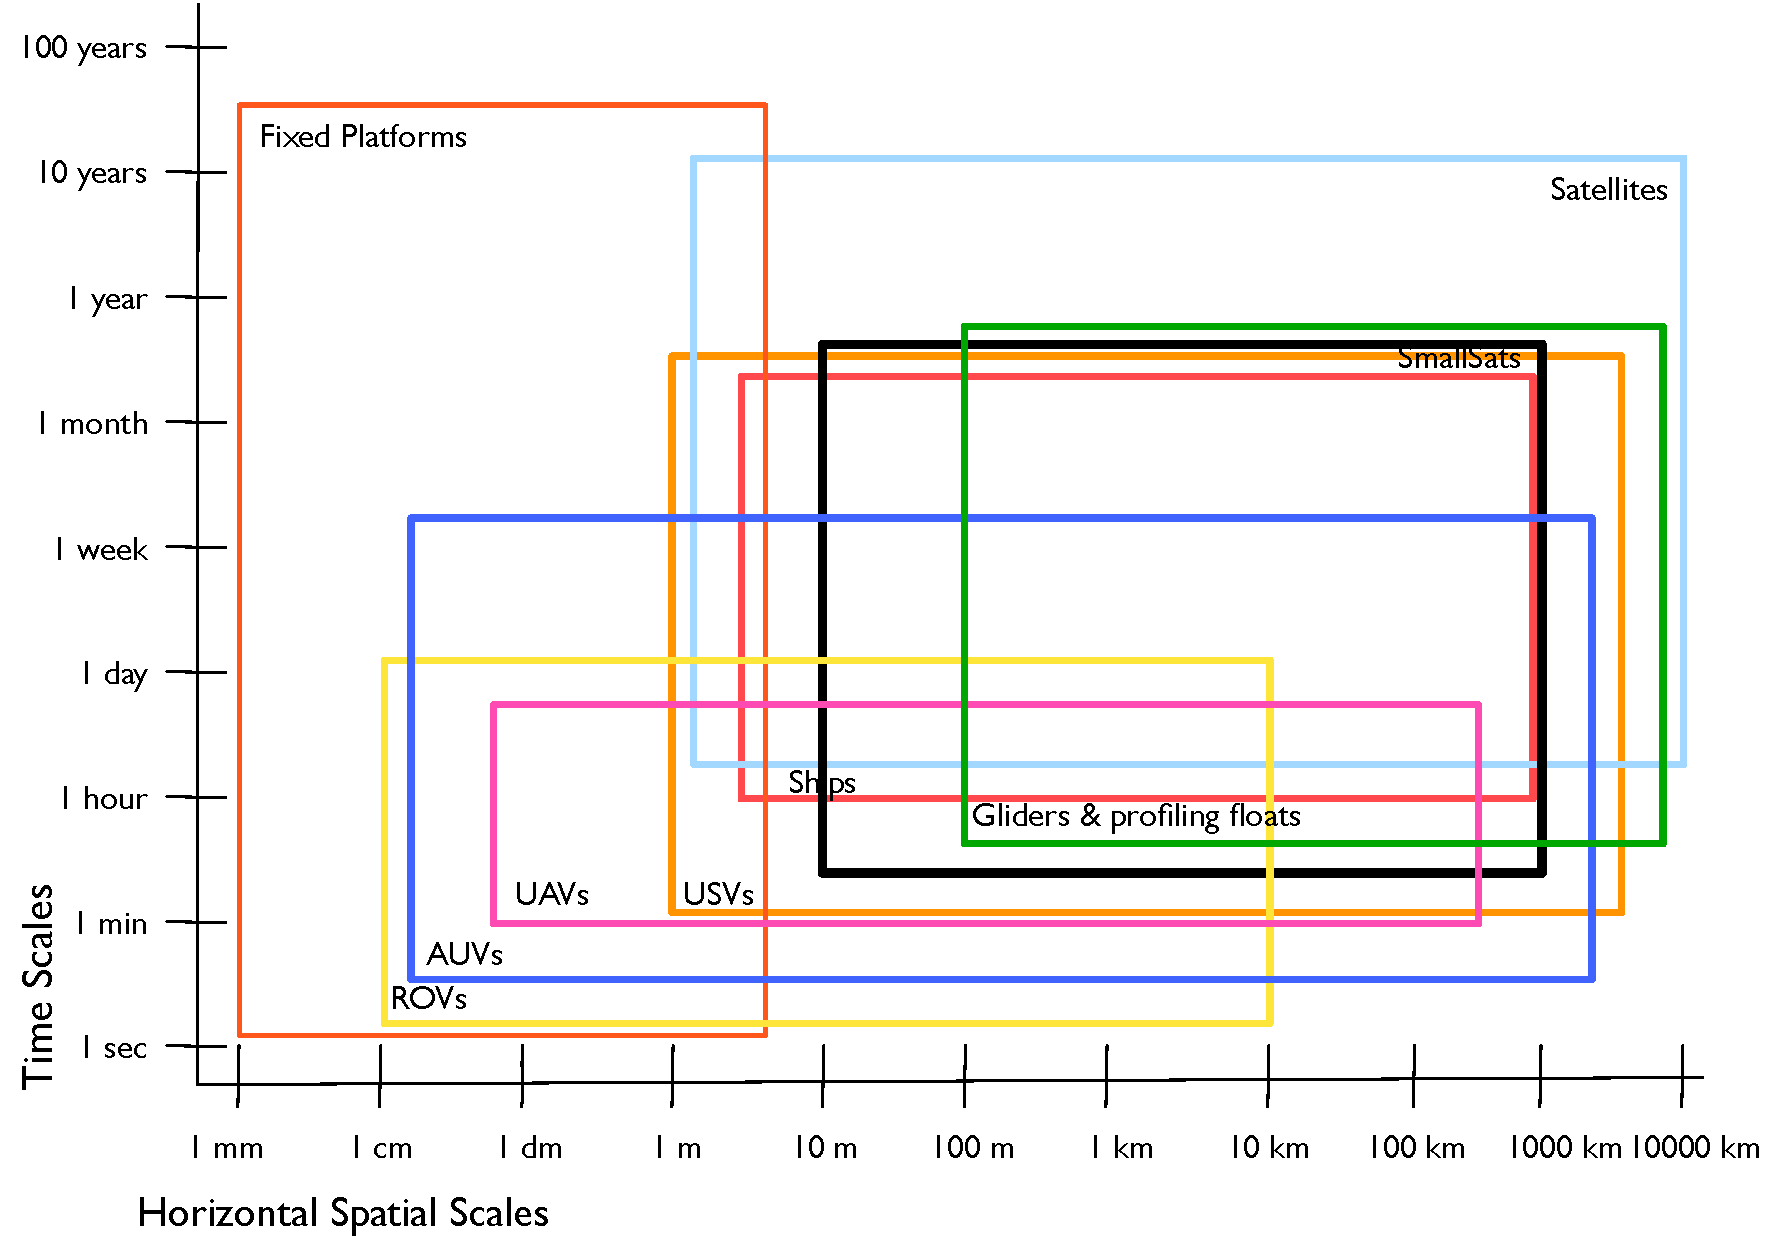
\includegraphics[width=0.7\textwidth]{fig/platform-capabilities.pdf}
  \caption{While \smle's do not occupy a unique position in ocean
    observation, overlapping a range of other assets, their capability
    for controlled observations along institutional lines is a
    harbringer of complementary views of the earths oceans. Figure
    modified from \cite{haury78}. \kc{Note this is a placeholder}}
  \label{fig:platforms}
\end{figure}


\begin{figure}[!t]
  \centering
  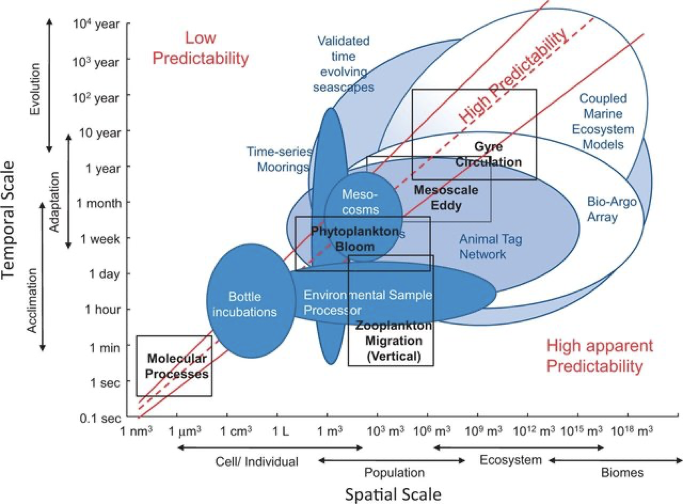
\includegraphics[width=0.7\textwidth]{fig/bio-processes.png}
  \caption{\kc{Note this is also a placeholder -- from Ajit}}
  \label{fig:platforms1}
\end{figure}

\begin{figure}[!t]
  \centering
  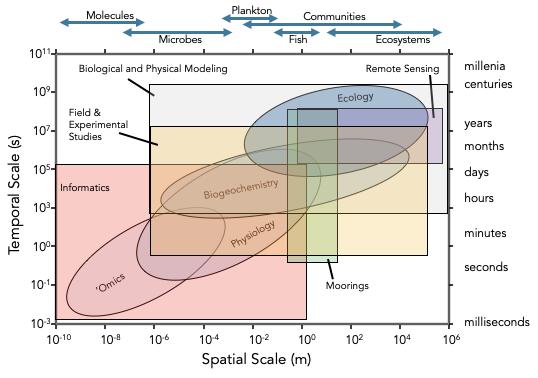
\includegraphics[width=0.7\textwidth]{fig/spatio-temporal.png}
  \caption{\kc{Note this is also a placeholder -- from Ajit}}
  \label{fig:platforms2}
\end{figure}


% Trace the advent of scientific instrumentation which morphed into
% floats, into gliders and powered AUVs.

\begin{enumerate} 

  % \item articulate the various 'robotic' vehicles, mobile and
  %   immobile. Keep this general, so even a buoy is a robotic sensing
  %   platform

  \item how an ensemble of vehicles can extend the “reach" of the
    human senses onboard the ship and perhaps even from shore with
    high bandwidth comms -- extend the above to not just water-column,
    but benthic work (where I know very little)

  \item Show the figure of which robotic assets are viable for what
    kinds of observation. Overlay bio-physical processes which are
    appropriate and discuss at length why these assets suit those
    specific observations.

  \item Articulate how robots have 'extended the human senses' from
    ship and shore to provide new ways of observing the ocean

  \item In brief -- examples of Machine Learning and other forms of AI
    which can help and how (see below). Machine Learning offline or
    even inline in the perspective of “discovery"

  \item How systematic observation, as against point measurements
    (i.e. dipping a rosette) and using extrapolation, can help. What
    kinds of signals are being missed

  \item Harshness of the environment and operational issues of being
    at sea for sustained presence

\end{enumerate}
